% Tento soubor nahraďte vlastním souborem s přílohami (nadpisy níže jsou pouze pro příklad)

% Pro kompilaci po částech (viz projekt.tex), nutno odkomentovat a upravit
%\documentclass[../projekt.tex]{subfiles}
%\begin{document}

% Umístění obsahu paměťového média do příloh je vhodné konzultovat s vedoucím
\chapter{Obsah přiloženého paměťového média}

\begin{itemize}
    \item \texttt{application/} -- adresář obsahující firmware digitálního záznamníku, včetně vygenerované HTML a Doxygen dokumentace
    \begin{itemize}
        \item \texttt{src/} -- adresář obsahující zdrojové soubory firmwaru digitálního záznamníku
        \item \texttt{include/} -- adresář obsahující hlavičkové soubory firmwaru digitálního záznamníku
        \item \texttt{doc/} -- adresář obsahující LaTeX a HTML Doxygen dokumentaci firmwaru digitálního záznamníku
        \item součástí projektu jsou nutné externí knihovny a moduly, které jsou potřeba k sestavení projektu, tyto celky byly převzdaty z MCUXpresso SDK
    \end{itemize}
    \item \texttt{hardware/} -- adresář s projektem expanzní desky: schématy zapojení, návrhem PCB, seznamem součástek (BOM) a schématem v PDF

    \begin{itemize}
        \item \texttt{expansion_shield/} -- adresář obsahující KiCAD projekt expanzní desky.
        \begin{itemize}
            \item \texttt{extension\_shield.kicad\_pro} -- hlavní projektový soubor KiCadu pro návrh expanzní desky
        \end{itemize}
        \item \texttt{BOM.txt} -- seznam komponent expanzní desky digitálního záznamníku
        \item \texttt{schematik.pdf} -- schématik realizované expanzní desky
    \end{itemize}

    
    \item \texttt{thesis/} -- adresář obsahující text technické zprávy k bakalářské práci, včetně obrázků a diagramů

    \begin{itemize}
        \item \texttt{xdolak09-bthesis.pdf} -- finální text technické zprávy k bakalářské práci
        \item \texttt{xdolak09-bthesis-src.zip} -- archiv se zdrojovými soubory zprávy, včetně všech použitých obrázků
    \end{itemize}
    
    
    \item \texttt{power\_consumption/} -- data z analýzy spotřeby energie, změřená pomocí Power Profiler Kit II od společnosti Nordic Semiconductors, součástí složky je také soubor \texttt{README.md} s popisem jednotlivých měření a souborů

    \item \texttt{powerloss\_detection/} -- data z analýzy chování digitálního záznamníku při ztrátě napájecího napětí zaznamenaná pomocí Saleae Logic 16 Pro, složka rovněž obsahuje soubor \texttt{README.md} s vysvětlením struktury a významu jednotlivých souborů
    
    \item \texttt{tests/} -- adresář obsahující testovací skripty, testovací soubory a výstupy ze statické analýzy kódu pomocí nástroje PC-lint Plus

    \item \texttt{misc/} -- složka obsahující nezařazené soubory, například obrázky k README

    \item \texttt{manual.pdf} -- manuál k použití digitálního záznamníku
    \item \texttt{video-ukazka.mp4} -- video ukázka použití digitálního záznamníku ve formátu MP4
    \item \texttt{video-ukazka.mov} -- video ukázka použití digitálního záznamníku ve formátu MOV
    \item \texttt{README.md} -- úvodní soubor s popisem projektu, instalací a způsobem použití
\end{itemize}

Celý obsah přiloženého paměťového média je dostupný prostřednictvím cloudového úložiště Nextcloud na adrese: \url{https://nextcloud.fit.vutbr.cz/s/xgZG6ZdZeccKQMC}.

\chapter{Schéma expanzní desky}
\vspace{-2em}
V této příloze je vložen schématický návrh expanzní desky, který byl vytvořen v programu KiCad 8 pro potřeby této práce.

%\clearpage
%\thispagestyle{empty}

\begin{figure}[H]
    \centering
    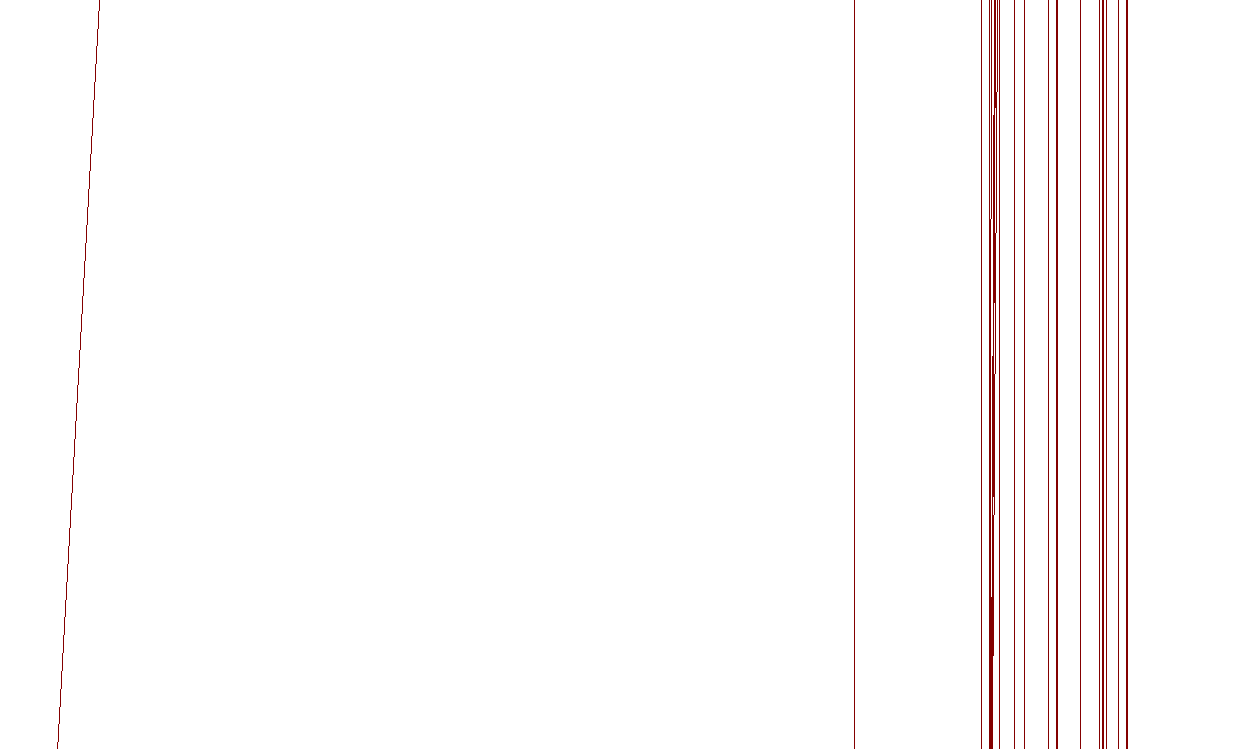
\includegraphics[width=0.95\textheight, angle=90]{obrazky-figures/circuits.pdf}
\end{figure}

%\clearpage
%\thispagestyle{empty}

\begin{figure}[H]
    \centering
    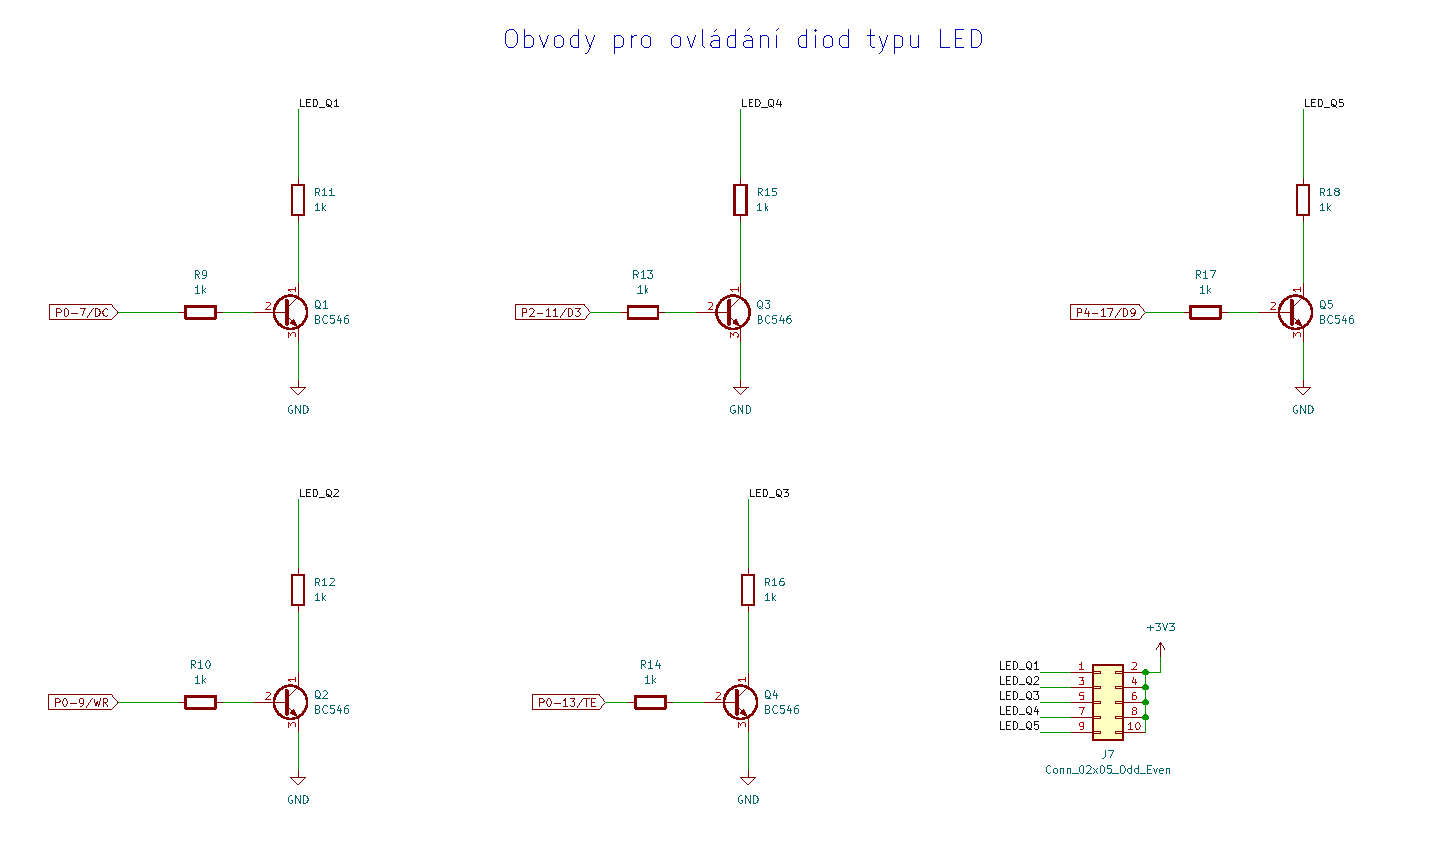
\includegraphics[width=1.00\textheight, angle=90]{obrazky-figures/diodes.pdf}
\end{figure}

%\clearpage
%\thispagestyle{empty}

\begin{figure}[H]
    \centering
    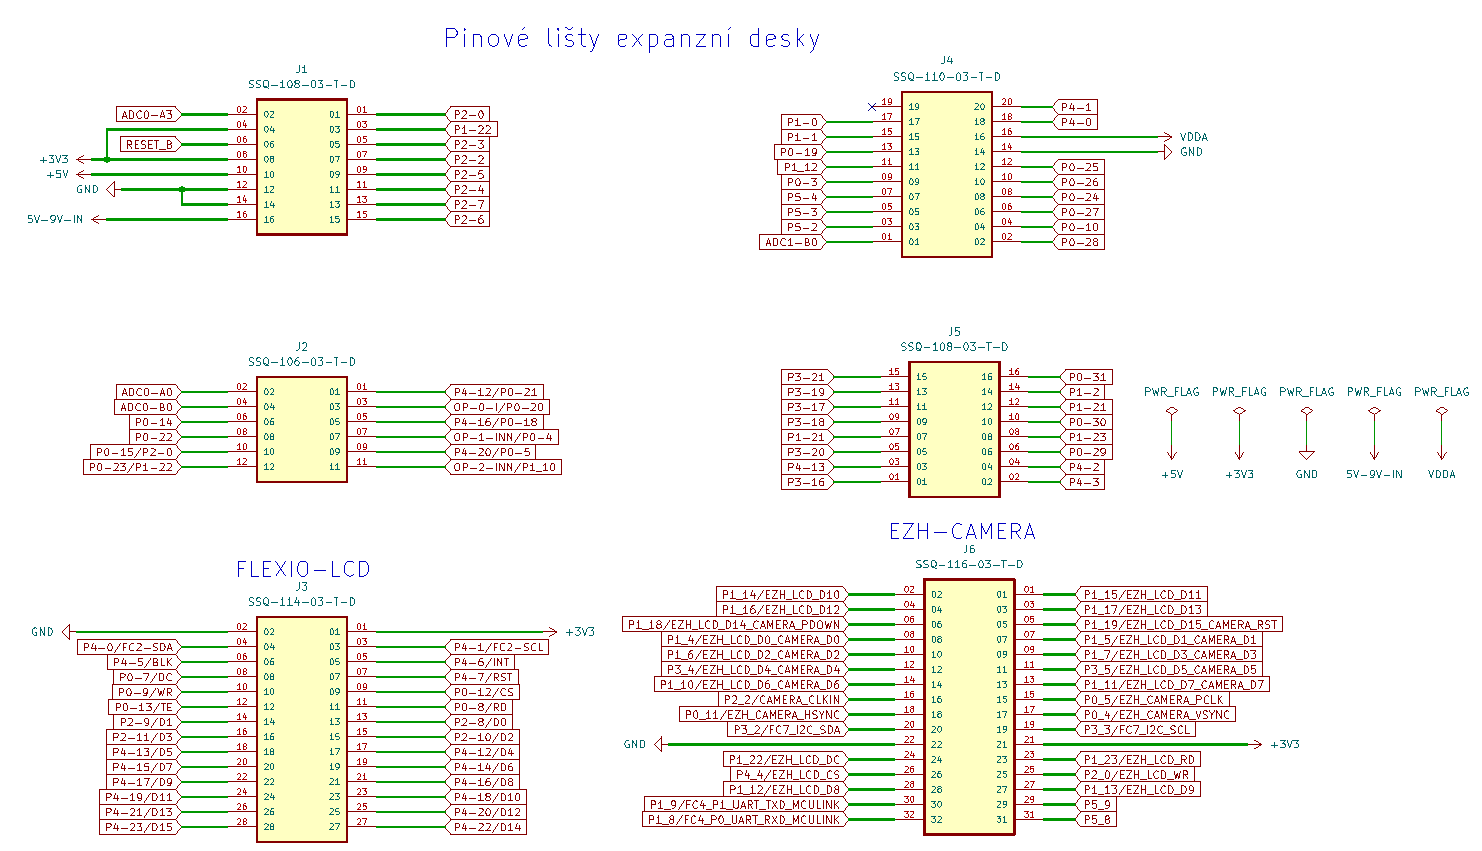
\includegraphics[width=1.00\textheight, angle=90]{obrazky-figures/pin-headers.pdf}
\end{figure}

\chapter{Layout expanzní desky}

\begin{figure}[H]
    \centering
    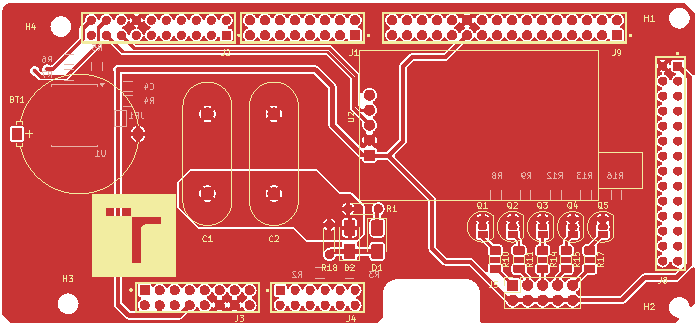
\includegraphics[width=0.67\textheight, angle=90]{obrazky-figures/extension_shield-brd-front.pdf}
    \caption{Layout expanzní desky -- přední strana}
    \label{fig:layout-front-big}
\end{figure}

\begin{figure}[H]
    \centering
    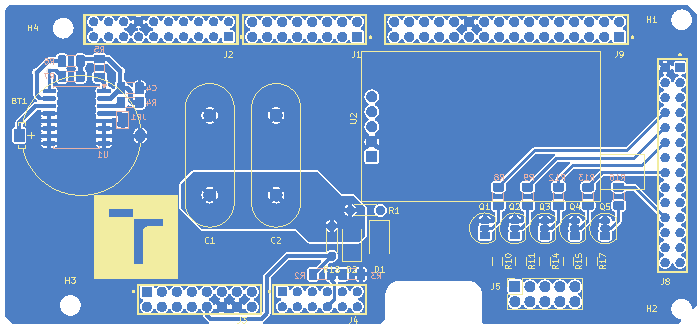
\includegraphics[width=0.67\textheight, angle=90]{obrazky-figures/extension_shield-brd-back.pdf}
    \caption{Layout expanzní desky -- spodní strana}
    \label{fig:layout-back-big}
\end{figure}

\chapter{Seznam použitých komponent}

\begin{table}[htbp]
    \centering
    \caption{Přehled použitých komponent}
    \label{tab:bom}
    \begin{tabularx}{\textwidth}{|X|X|c|}
        \hline
        \textbf{Komponenta} & \textbf{Hodnota / Popis} & \textbf{Počet} \\
        \hline
        NXP FRDM-MCXN947    & vývojová deska                 & 1  \\ \hline
        SSQ-108-03-T-D      & 16-pinová lišta (Samtec)       & 2  \\ \hline
        SSQ-106-03-T-D      & 12-pinová lišta (Samtec)       & 1  \\ \hline
        SSQ-114-03-T-D      & 28-pinová lišta (Samtec)       & 1  \\ \hline
        SSQ-116-03-T-D      & 32-pinová lišta (Samtec)       & 1  \\ \hline
        SSQ-110-03-T-D      & 20-pinová lišta (Samtec)       & 1  \\ \hline
        M20-7830342         & 10-pinová lišta (Harwin)       & 1  \\ \hline
        DS3231M+            & Obvod reálného času             & 1  \\ \hline
        SCMR14G334SRBB0     & Superkondenzátor (\mbox{KYOCERA AVX})  & 1  \\ \hline
        RSX301L-30DDTE25    & Schottky dioda (ROHM)           & 1  \\ \hline
        BC546               & NPN tranzistor (ON Semi)        & 5  \\ \hline
        Bateriový box CR2032 & --                             & 1  \\ \hline
        THT rezistor        & $\SI{10}{\ohm}$                 & 1  \\ \hline
        SMD rezistor R1206  & $\SI{18}{\kilo\ohm}$            & 1  \\ \hline
        SMD rezistor R1206  & $\SI{33}{\kilo\ohm}$            & 1  \\ \hline
        SMD rezistor R1206  & $\SI{1}{\kilo\ohm}$             & 14 \\ \hline
        SMD kondenzátor R1206  & $\SI{1}{\nano\farad}$        & 1  \\ \hline
    \end{tabularx}
\end{table}

\chapter{Projekt digitálního záznamníku}
Digitální záznamník je možné dále rozšířit nebo upravit dle konkrétních požadavků. Celý projekt, včetně implementace firmwaru, návrhu expanzní desky i veškeré dokumentace, je veřejně dostupný na platformě GitHub.

\begin{itemize}
    \item Odkaz na GitHub repozitář je \url{https://github.com/Doly02/nxp-mcxn947-datalogger}
\end{itemize}
    
\chapter{Použité nástroje}

\begin{itemize}
    \item \textbf{MCUXpresso IDE} ve verzi 11.10.0, jež bylo využito jako hlavní vývojové prostředí pro implementaci firmwaru digitálního záznamníku.
    \item \textbf{NXP SDK FRDM-MCXN947} ve verzi 2.16.000 včetně kterého jsou ovladače pro desku \textbf{FRDM-MCXN947}, knihovna \textbf{FATFS}, operační systém reálného času \textbf{FreeRTOS} a~moduly \textbf{Mass Storage}, \textbf{MMC} a~\textbf{USB}.
    \item \textbf{MCU LinkServer}, který byl použitý pro nahrávání a ladění firmwaru.
    \item \textbf{nRF Connect for Desktop} od \textbf{Nordic Semiconductor} pro měření spotřeby digitálního záznamníku pomocí \textbf{Power Profiler Kit II}.
    \item \textbf{Logic} ve verzi 2.4.22 pro pozorování signálů digitálního záznamníku pomocí logického analyzátoru \textbf{Saleae Logic Pro~16}.
    \item \textbf{GitHub} pro verzování firmwaru digitálního záznamníku a~technické zprávy.
    \item \textbf{KiCAD 8} pro návrh expanzní desky digitálního záznamníku.
    \item \textbf{PC-lint Plus} ve verzi 2.2 pro statickou analýzu zdrojového kódu. 
    \item \textbf{Doxygen} pro generování HTML a~LaTeX dokumentace zdrojového kódu.
    \item \textbf{Overleaf} pro úpravu zdrojových souborů technické zprávy.
    \item \textbf{Draw.io} pro tvorbu diagramů, které jsou součástí technické zprávy.
    \item \textbf{ChatGPT}, který byl využit pro návrhy vylepšení struktury a~formulace vět v~technické zprávě.
\end{itemize}

% Pro kompilaci po částech (viz projekt.tex) nutno odkomentovat
%\end{document}
